\paragraph{QuizziPedia::Front-End::Controllers::LoginController}
\begin{figure} [ht]
	\centering
	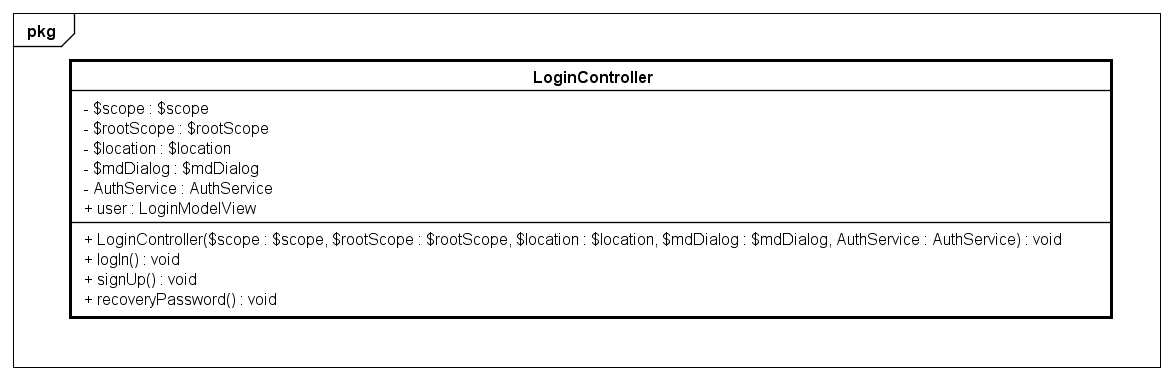
\includegraphics[scale=0.45]{UML/Classi/Front-End/QuizziPedia_Front-end_Controller_LoginController.png}
	\caption{QuizziPedia::Front-End::Controllers::LoginController}
\end{figure} \FloatBarrier
\begin{itemize}
	\item \textbf{Descrizione}: questa classe permette di gestire l'autenticazione dell'utente al sistema; 
	\item \textbf{Utilizzo}: fornisce le funzionalità di autenticazione al sistema, compresa la gestione di situazioni di errore di autenticazione;
	\item \textbf{Relazione con altre classi}:
	\begin{itemize}
		\item \textit{IN} \texttt{LoginModelView}: classe di tipo modelview la cui istanzazione è contenuta all'interno della variabile di ambiente \$scope di \textit{Angular.js\ped{G}}. All'interno di essa sono presenti le variabili e i metodi necessari per il \textit{Two-Way Data-Binding\ped{G}} tra la view \texttt{LoginView} e il controller \texttt{LoginController};
		\item \textit{IN} \texttt{AuthService}: questa classe permette di gestire la registrazione e l'autenticazione di un utente;
	\end{itemize}
	\item \textbf{Attributi}:
	\begin{itemize}
		\item \texttt{-} \texttt{\$scope: \$scope} \\
		Campo dati contenente un riferimento all’oggetto \$scope creato da \textit{Angular\ped{G}}. Viene utilizzato come mezzo di comunicazione tra il controller e la view. Contiene gli oggetti che definiscono il viewmodel e il model dell’applicazione;
		\item \texttt{-} \texttt{\$location: \$location} \\
		Campo dati contenente un riferimento al servizio creato da \textit{Angular\ped{G}} che permette di accedere alla barra degli indirizzi del \textit{browser\ped{G}}, i cambiamenti all’URL nella barra degli indirizzi si riflettono in questo oggetto e viceversa;
		\item \texttt{-} \texttt{\$mdDialog: \$mdDialog} \\
		Campo dati contenente un riferimento al servizio della libreria \textit{Material for Angular\ped{G}} che permette di creare delle componenti a popup;
		\item \texttt{-} \texttt{AuthService: AuthService} \\
		Campo dati contenente un riferimento al servizio che si occupa della gestione delle informazioni legate all’autenticazione. Viene utilizzato il metodo \texttt{logIn} di \$texttt{AuthService} a cui vengono passati i parametri \texttt{username} e \texttt{password};
		\item \texttt{+} \texttt{user: LoginModelView} \\
		Oggetto di tipo \texttt{LoginModelView}. All'interno di esso sono presenti le variabili e i metodi necessari per il \textit{Two-Way Data-Binding\ped{G}} tra la view \texttt{LoginView} e il controller \texttt{LoginController};
	\end{itemize}
	\item \textbf{Metodi}:
	\begin{itemize}
		\item \texttt{+} \texttt{LoginController(\$scope: \$scope, \$rootScope: \$rootScope, \$location: \$location, \$mdDialog: \$mdDialog, AuthService: AuthService)} \\
		Metodo costruttore della classe: \\
		\textbf{Parametri}:
			\begin{itemize}
				\item \texttt{\$scope: \$scope} \\
				Parametro contenente un riferimento all’oggetto \$scope creato da \textit{Angular\ped{G}}. Viene utilizzato come mezzo di comunicazione tra il controller e la view. Contiene gli oggetti che definiscono il viewmodel e il model dell’applicazione;
				\item \texttt{\$location: \$location} \\
				Parametro contenente un riferimento al servizio creato da \textit{Angular\ped{G}} che permette di accedere alla barra degli indirizzi del \textit{browser\ped{G}}, i cambiamenti all’URL nella barra degli indirizzi si riflettono in questo oggetto e viceversa;
				\item \texttt{\$mdDialog: \$mdDialog} \\
				Parametro contenente un riferimento al servizio della libreria \textit{Material for Angular\ped{G}} che permette di creare delle componenti a popup;
				\item \texttt{AuthService: AuthService} \\
				Parametro contenente un riferimento al servizio che si occupa della gestione delle informazioni legate all’autenticazione. Viene utilizzato il metodo \texttt{logIn} di \$texttt{AuthService} a cui vengono passati i parametri \texttt{username} e \texttt{password};
			\end{itemize}
		\item \texttt{+} \texttt{logIn(): void} \\
		Metodo che richiama il metodo \texttt{Login} del service \texttt{AuthService} passandogli \texttt{username} e \texttt{password}. Nel caso di buona riuscita dell'operazione viene effettuato il redirect alla homepage dell'applicazione. Nel caso in cui invece avvenga un errore, viene mostrato a video il messaggio di errore;
		\item \texttt{+} \texttt{signUp(): void} \\
		Metodo che gestisce l’evento click sul pulsante di registrazione. Effettua il redirect alla pagina di registrazione;
		\item \texttt{+} \texttt{recoveryPassword(): void} \\
		Metodo che gestisce l’evento click sul pulsante di recupero password. Effettua il redirect alla pagina per il recupero della password; 
	\end{itemize}
\end{itemize}

\paragraph{QuizziPedia::Front-End::Controllers::SignUpController}
\begin{figure} [ht]
	\centering
	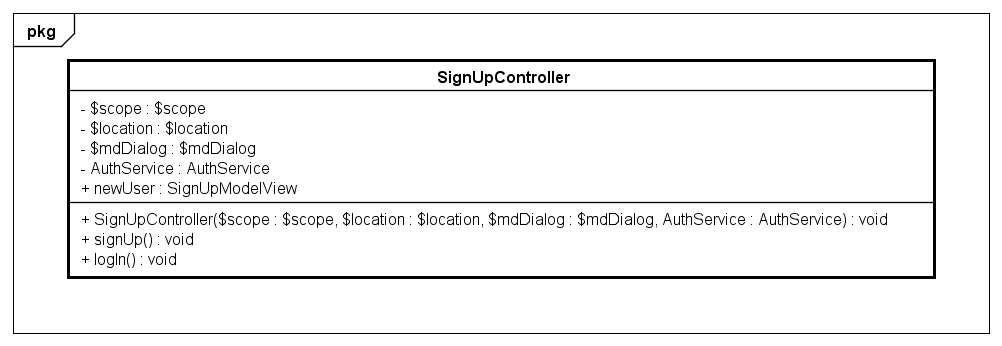
\includegraphics[scale=0.45]{UML/Classi/Front-End/QuizziPedia_Front-end_Controller_SignUpController.png}
	\caption{QuizziPedia::Front-End::Controllers::SignUpController}
\end{figure} \FloatBarrier
\begin{itemize}
	\item \textbf{Descrizione}: questa classe permette di gestire la registrazione di un utente al sistema;
	\item \textbf{Utilizzo}: fornisce le funzionalità di registrazione di un utente al sistema;
	\item \textbf{Relazione con altre classi}:
	\begin{itemize}
		\item \textit{IN} \texttt{SignUpModelView}: classe di tipo modelview la cui istanzazione è contenuta all'interno della variabile di ambiente \$scope di \textit{Angular.js\ped{G}}. All'interno di essa sono presenti le variabili e i metodi necessari per il \textit{Two-Way Data-Binding\ped{G}} tra la view \texttt{SignUpView} e il controller \texttt{SignUpController};
		\item \textit{IN} \texttt{AuthService}: questa classe permette di gestire la registrazione e l'autenticazione di un utente;
	\end{itemize}
	\item \textbf{Attributi}:
	\begin{itemize}
		\item \texttt{-} \texttt{\$scope: \$scope} \\
		Campo dati contenente un riferimento all’oggetto \$scope creato da \textit{Angular\ped{G}}. Viene utilizzato come mezzo di comunicazione tra il controller e la view. Contiene gli oggetti che definiscono il viewmodel e il model dell’applicazione;
		\item \texttt{-} \texttt{\$location: \$location} \\
		Campo dati contenente un riferimento al servizio creato da \textit{Angular\ped{G}} che permette di accedere alla barra degli indirizzi del \textit{browser\ped{G}}, i cambiamenti all’URL nella barra degli indirizzi si riflettono in questo oggetto e viceversa;
		\item \texttt{-} \texttt{\$mdDialog: \$mdDialog} \\
		Campo dati contenente un riferimento al servizio della libreria \textit{Material for Angular\ped{G}} che permette di creare delle componenti a popup;
		\item \texttt{-} \texttt{AuthService: AuthService} \\
		Campo dati contenente un riferimento al servizio che si occupa della gestione delle informazioni legate all’autenticazione. Viene utilizzato il metodo \texttt{signUp} di \$texttt{AuthService} a cui viene passato come parametro un oggetto di tipo \texttt{SignUpModelView};
		\item \texttt{+} \texttt{newUser: SignUpModelView} \\
		Oggetto di tipo \texttt{SignUpModelView}. All'interno di esso sono presenti le variabili e i metodi necessari per il \textit{Two-Way Data-Binding\ped{G}} tra la view \texttt{SignUpView} e il controller \texttt{SignUpController};
	\end{itemize}
	\item \textbf{Metodi}:
	\begin{itemize}
		\item \texttt{+} \texttt{SignUpController(\$scope: \$scope, \$location: \$location, \$mdDialog: \$mdDialog, AuthService: AuthService)} \\
		Metodo costruttore della classe: \\
		\textbf{Parametri}:
		\begin{itemize}
			\item \texttt{\$scope: \$scope} \\
			Parametro contenente un riferimento all’oggetto \$scope creato da \textit{Angular\ped{G}}. Viene utilizzato come mezzo di comunicazione tra il controller e la view. Contiene gli oggetti che definiscono il viewmodel e il model dell’applicazione;
			\item \texttt{\$location: \$location} \\
			Parametro contenente un riferimento al servizio creato da \textit{Angular\ped{G}} che permette di accedere alla barra degli indirizzi del \textit{browser\ped{G}}, i cambiamenti all’URL nella barra degli indirizzi si riflettono in questo oggetto e viceversa;
			\item \texttt{\$mdDialog: \$mdDialog} \\
			Parametro contenente un riferimento al servizio della libreria \textit{Material for Angular\ped{G}} che permette di creare delle componenti a popup;
			\item \texttt{AuthService: AuthService} \\
			Campo dati contenente un riferimento al servizio che si occupa della gestione delle informazioni legate all’autenticazione. Viene utilizzato il metodo \texttt{logIn} di \$texttt{AuthService} a cui vengono passati i parametri \texttt{username} e \texttt{password};
		\end{itemize}
		\item \texttt{+} \texttt{signUp(): void} \\
		Metodo che richiama il metodo \texttt{signUp} del service \texttt{AuthService} passandogli un oggetto di tipo \texttt{SignUpModelView}. Nel caso di buona riuscita dell'operazione viene mostrato un messaggio di successo. Con l'azione di click sul bottone presentato dal messaggio di successo è possibile effettuare il redirect alla pagina di login dell'applicazione. Nel caso in cui invece avvenga un errore, viene mostrato a video il messaggio di errore;
		\item \texttt{+} \texttt{logIn(): void} \\
		Metodo che gestisce l’evento click sul pulsante di login. Effettua il redirect alla pagina di login;
	
	\end{itemize}
\end{itemize}

\paragraph{QuizziPedia::Front-End::Controllers::HomeController}
\begin{figure} [ht]
	\centering
	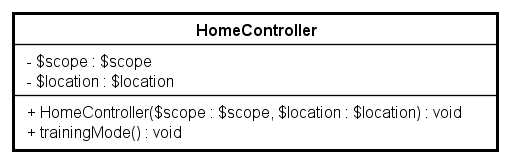
\includegraphics[scale=0.45]{UML/Classi/Front-End/QuizziPedia_Front-end_Controller_HomeController.png}
	\caption{QuizziPedia::Front-End::Controllers::HomeController}
\end{figure} \FloatBarrier
\begin{itemize}
	\item \textbf{Descrizione}: questa classe permette di gestire la home page;
	\item \textbf{Utilizzo}: fornisce tutte le informazioni da mostrare nella homepage;
	\item \textbf{Relazione con altre classi}:
	\begin{itemize}
		\item \textit{IN} \texttt{HomeModelView}: classe di tipo modelview la cui istanzazione è contenuta all'interno della variabile di ambiente \$scope di \textit{Angular.js\ped{G}}. All'interno di essa sono presenti le variabili e i metodi necessari per il \textit{Two-Way Data-Binding\ped{G}} tra la view \texttt{HomeView} e il controller \texttt{HomeController};
	\end{itemize}
	\item \textbf{Attributi}:
	\begin{itemize}
		\item \texttt{-} \texttt{\$scope: \$scope} \\
		Campo dati contenente un riferimento all’oggetto \$scope creato da \textit{Angular\ped{G}}, viene utilizzato come mezzo di comunicazione tra il controller e la view. Contiene gli oggetti che definiscono il model dell’applicazione;
		\item \texttt{-} \texttt{\$location: \$location} \\
		Campo dati contenente un riferimento al servizio creato da \textit{Angular\ped{G}} che permette di accedere alla barra degli indirizzi del \textit{browser\ped{G}}, i cambiamenti all’URL nella barra degli indirizzi si riflettono in questo oggetto e viceversa;
	\end{itemize}
	\item \textbf{Metodi}:
	\begin{itemize}
		\item \texttt{+} \texttt{HomeController(\$scope: \$scope, \$location: \$location)} \\
		Metodo costruttore della classe: \\
		\textbf{Parametri}:
		\begin{itemize}
			\item \texttt{\$scope: \$scope} \\
			Parametro contenente un riferimento all’oggetto \$scope creato da \textit{Angular\ped{G}}. Viene utilizzato come mezzo di comunicazione tra il controller e la view. Contiene gli oggetti che definiscono il viewmodel e il model dell’applicazione;
			\item \texttt{\$location: \$location} \\
			Parametro contenente un riferimento al servizio creato da \textit{Angular\ped{G}} che permette di accedere alla barra degli indirizzi del \textit{browser\ped{G}}, i cambiamenti all’URL nella barra degli indirizzi si riflettono in questo oggetto e viceversa;
		\end{itemize}
		\item \texttt{+} \texttt{trainingMode(): void} \\
		Metodo che gestisce l’evento click sul pulsante di allenamento. Effettua il redirect alla pagina di allenamento; 
	\end{itemize}
\end{itemize}

\paragraph{QuizziPedia::Front-End::Controllers::SearchController}
\begin{figure} [ht]
	\centering
	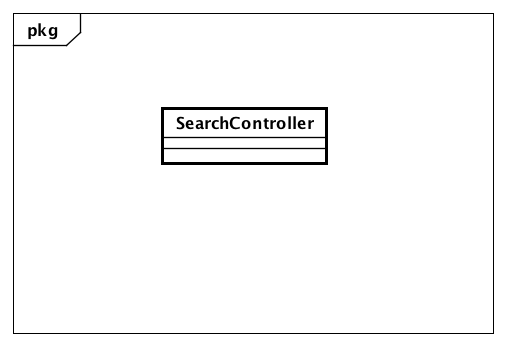
\includegraphics[scale=0.45]{UML/Classi/Front-End/QuizziPedia_Front-end_Controller_SearchController.png}
	\caption{QuizziPedia::Front-End::Controllers::SearchController}
\end{figure} \FloatBarrier
\begin{itemize}
	\item \textbf{Descrizione}: questa classe permette di gestire la ricerca di questionari e utenti all'interno dell'applicazione;
	\item \textbf{Utilizzo}: fornisce all'utente le funzionalità di ricerca per utenti e questionari;
	\item \textbf{Relazione con altre classi}:
	\begin{itemize}
		\item \textit{IN} \texttt{ResultsModelView}: view contenente i risultati della ricerca effettuata, sia gli utenti che i questionari;
		\item \textit{IN} \texttt{SearchService}: questa classe permette di eseguire una ricerca tra i questionari e gli utenti presenti ritornando un \textit{Object} contenente i risultati di tale operazione;
		\item \textit{IN} \texttt{QuizService}: questa classe permette di ottenere i dati di un quiz tramite delle parole chiave inserite dall'utente nella barra di ricerca. Permette inoltre di iscriversi ad un questionario;
	\end{itemize}
	\item \textbf{Attributi}:
	\begin{itemize}
		\item \texttt{-} \texttt{\$scope: \$scope} \\
		Campo dati contenente un riferimento all’oggetto \$scope creato da \textit{Angular\ped{G}}, viene utilizzato come mezzo di comunicazione tra il controller e la view. Contiene gli oggetti che definiscono il model dell’applicazione;
		\item \texttt{-} \texttt{\$location: \$location} \\
		Campo dati contenente un riferimento al servizio creato da \textit{Angular\ped{G}} che permette di accedere alla barra degli indirizzi del \textit{browser\ped{G}}, i cambiamenti all’URL nella barra degli indirizzi si riflettono in questo oggetto e viceversa;
		\item \texttt{-} \texttt{\$mdDialog: \$mdDialog} \\
		Campo dati contenente un riferimento al servizio della libreria \textit{Material for Angular\ped{G}} che permette di creare delle componenti a popup;
		\item \texttt{-} \texttt{SearchService: SearchService} \\
		Campo dati contenente un riferimento al servizio che si occupa della gestione delle informazioni legate alla ricerca. Viene utilizzato il metodo \texttt{search} di \$texttt{SearchService} a cui viene passato come parametro la stringa di ricerca;
		\item \texttt{-} \texttt{QuizService: QuizService} \\
		Campo dati contenente un riferimento al servizio che si occupa della gestione delle informazioni legate ai questionari. Viene utilizzato il metodo \texttt{subscribeQuestionnaire} di \$texttt{QuizService} per iscrivere un utente ad un questionario;
		\item \texttt{+} \texttt{result: SearchModelView} \\
		Oggetto di tipo \texttt{SearchModelView}. All'interno di esso sono presenti le variabili e i metodi necessari per il \textit{Two-Way Data-Binding\ped{G}} tra la view \texttt{ResultView} e il controller \texttt{SearchController};
	\end{itemize}
	\item \textbf{Metodi}:
	\begin{itemize}
		\item \texttt{+} \texttt{SearchController(\$scope: \$scope, \$location: \$location, \$mdDialog: \$mdDialog, SearchService: SearchService)} \\
		Metodo costruttore della classe. Viene eseguita la ricerca per poter poi popolare il campo dati \texttt{result}. \\
		\textbf{Parametri}:
		\begin{itemize}
			\item \texttt{\$scope: \$scope} \\
			Parametro contenente un riferimento all’oggetto \$scope creato da \textit{Angular\ped{G}}. Viene utilizzato come mezzo di comunicazione tra il controller e la view. Contiene gli oggetti che definiscono il viewmodel e il model dell’applicazione;
			\item \texttt{\$location: \$location} \\
			Parametro contenente un riferimento al servizio creato da \textit{Angular\ped{G}} che permette di accedere alla barra degli indirizzi del \textit{browser\ped{G}}, i cambiamenti all’URL nella barra degli indirizzi si riflettono in questo oggetto e viceversa;
			\item \texttt{\$mdDialog: \$mdDialog} \\
			Parametro contenente un riferimento al servizio della libreria \textit{Material for Angular\ped{G}} che permette di creare delle componenti a popup;
			\item \texttt{SearchService: SearchService} \\
			Parametro contenente un riferimento al servizio che si occupa della gestione delle informazioni legate alla ricerca. Viene utilizzato il metodo \texttt{search} di \$texttt{SearchService} a cui viene passato come parametro la stringa di ricerca;
		\end{itemize} 
		\item \texttt{-} \texttt{getSearch(stringSearch: String): SearchModelView} \\
		Metodo che esegue la ricerca utilizzando un metodo fornito dalla classe SearchService. \\
		\textbf{Parametri}:
		\begin{itemize}
			\item \texttt{stringSearch: String} \\
			Parametro contenente la stringa della quale effettuare la ricerca;
		\end{itemize} 
		\item \texttt{+} \texttt{goToUser(idUser: String): void} \\
		Metodo che gestisce l’evento click sul bottone per visualizzare il profilo dell'utente selezionato. Effettua il redirect alla pagina dell'utente.\\
		\textbf{Parametri}:
		\begin{itemize}
			\item \texttt{idUser: String} \\
			Parametro contenente l'id dell'utente di cui si vuole visualizzare il profilo;
		\end{itemize} 
		\item \texttt{+} \texttt{registrationToQuiz(idQuiz: String): void} \\
		Metodo che gestisce l’evento click sul pulsante di registrazione al questionario.\\
		\textbf{Parametri}:
		\begin{itemize}
			\item \texttt{idQuiz: String} \\
			Parametro contenente l'id del questionario di cui si vuole effettuare l'iscrizione;
		\end{itemize} 
	\end{itemize}
\end{itemize}

\paragraph{QuizziPedia::Front-End::Controllers::ProfileManagementController}
\begin{figure} [ht]
	\centering
	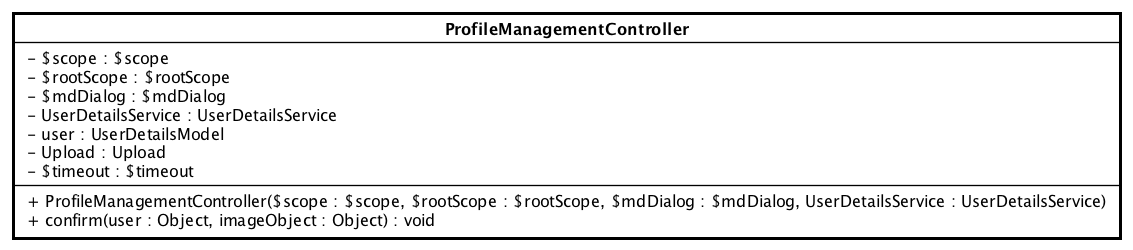
\includegraphics[scale=0.45]{UML/Classi/Front-End/QuizziPedia_Front-end_Controller_ProfileManagementController.png}
	\caption{QuizziPedia::Front-End::Controllers::ProfileManagementController}
\end{figure} \FloatBarrier
\begin{itemize}
	\item \textbf{Descrizione}: questa classe permette di gestire il profilo personale di un utente; 
	\item \textbf{Utilizzo}: fornisce le funzionalità all'utente per poter gestire i propri dati;
	\item \textbf{Relazione con altre classi}:
	\begin{itemize}
		\item \textit{IN} \texttt{ProfileManagementModelView}: classe di tipo modelview la cui istanzazione è contenuta all'interno della variabile di ambiente \$scope di \textit{Angular.js\ped{G}}. All'interno di essa sono presenti le variabili e i metodi necessari per il \textit{Two-Way Data-Binding\ped{G}} tra la view \texttt{ProfileManagementView} e il controller \texttt{ProfileManagementController};
		\item \textit{IN} \texttt{UserDetailsService}: questa classe permette di ottenere i dati personali degli utenti;
		\item \textit{IN} \texttt{UserDetailsModel}: questa classe rappresenta il tipo dell'utente autenticato della pagina; 
	\end{itemize}
	\item \textbf{Attributi}:
	\begin{itemize}
		\item \texttt{-} \texttt{\$scope: \$scope} \\
		Campo dati contenente un riferimento all’oggetto \$scope creato da \textit{Angular\ped{G}}, viene utilizzato come mezzo di comunicazione tra il controller e la view. Contiene gli oggetti che definiscono il model dell’applicazione;
		\item \texttt{-} \texttt{\$rootScope: \$rootScope} \\
		Campo dati contenente il riferimento all'oggetto globale \$rootScope creato da \textit{Angular\ped{G}}. Viene utilizzato per rendere accessibile a tutti i controller e a tutte le view l'oggetto \texttt{UserDetailsModel};
		\item \texttt{-} \texttt{\$mdDialog: \$mdDialog} \\
		Campo dati contenente un riferimento al servizio della libreria \textit{Material for Angular\ped{G}} che permette di creare delle componenti a popup;		
		\item \texttt{-} \texttt{UserDetailsService: UserDetailsService}: \\
		Campo dati contenente un riferimento al servizio che si occupa della gestione delle informazioni legate agli utenti;
		\item \texttt{+} \texttt{user: UserDetailsModel}: \\
		Oggetto di tipo \texttt{UserDetailsModel}. Viene mantenuto all'interno del \$rootScope; 
	\end{itemize}
	\item \textbf{Metodi}:
	\begin{itemize}
		\item \texttt{+} \texttt{ProfileManagementController(\$scope: \$scope, \$rootScope: \$rootScope, \$mdDialog: \$mdDialog, UserDetailsService: UserDetailsService)} \\
		Metodo costruttore della classe. \\
		\textbf{Parametri}:
		\begin{itemize}
			\item \texttt{\$scope: \$scope} \\
			Parametro contenente un riferimento all’oggetto \$scope creato da \textit{Angular\ped{G}}. Viene utilizzato come mezzo di comunicazione tra il controller e la view. Contiene gli oggetti che definiscono il viewmodel e il model dell’applicazione;
			\item \texttt{\$rootScope: \$rootScope} \\
			Parametro contenente il riferimento all'oggetto globale \$rootScope creato da \textit{Angular\ped{G}}. Viene utilizzato per rendere accessibile a tutti i controller e a tutte le view l'oggetto \texttt{UserDetailsModel}. In questo caso viene utilizzato per aggiornare in \$rootScope l'oggetto che rappresenta l'utente autenticato all'interno dell'applicazione;
			\item \texttt{\$location: \$location} \\
			Parametro contenente un riferimento al servizio creato da \textit{Angular\ped{G}} che permette di accedere alla barra degli indirizzi del \textit{browser\ped{G}}, i cambiamenti all’URL nella barra degli indirizzi si riflettono in questo oggetto e viceversa;
			\item \texttt{\$mdDialog: \$mdDialog} \\
			Parametro contenente un riferimento al servizio della libreria \textit{Material for Angular\ped{G}} che permette di creare delle componenti a popup;
			\item \texttt{UserDetailsService: UserDetailsService} \\
			Parametro contenente un riferimento al servizio che si occupa della gestione delle informazioni legate all’utente;
		\end{itemize}
		\item \texttt{+} \texttt{confirm(): void} \\
		Metodo che gestisce l’evento click sul pulsante di conferma modifica. Aggiorna, in caso di modifiche, l'oggetto locale \texttt{UserDetailsModel}. Inoltre, utilizzando il metodo dell'\texttt{UserDetailsService}, aggiorna anche nel server i dati dell'utente.

	\end{itemize}
\end{itemize}

\paragraph{QuizziPedia::Front-End::Controllers::PasswordForgotController}
\begin{figure} [ht]
	\centering
	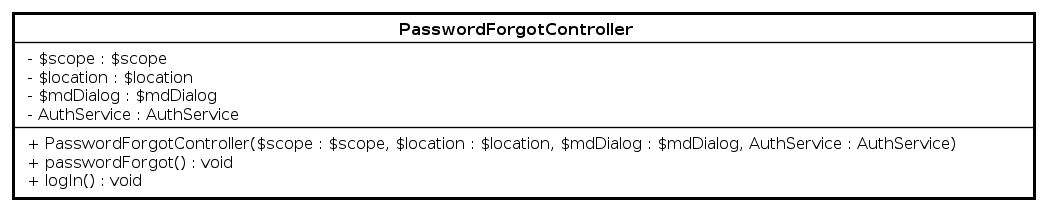
\includegraphics[scale=0.45]{UML/Classi/Front-End/QuizziPedia_Front-end_Controller_PasswordForgotController.png}
	\caption{QuizziPedia::Front-End::Controllers::PasswordForgotController}
\end{figure} \FloatBarrier
\begin{itemize}
	\item \textbf{Descrizione}: questa classe permette di gestire il ripristino della password dimenticata;
	\item \textbf{Utilizzo}: fornisce tutte le funzionalità per ripristinare la password dopo aver verificato l'identità dell'utente;
	\item \textbf{Relazione con altre classi}:
	\begin{itemize}
		\item \textit{IN} \texttt{PasswordForgotModelView}: classe di tipo modelview la cui istanzazione è contenuta all'interno della variabile di ambiente \$scope di \texttt{Angular.js}. All'interno di essa sono presenti le variabili e i metodi necessari per il \textit{Two-Way Data-Binding\ped{G}} tra la view \texttt{PasswordForgotView} e il controller \texttt{PasswordForgotController};
		\item \textit{IN} \texttt{AuthService}: questa classe permette di gestire la registrazione e l'autenticazione di un utente;
	\end{itemize}
	\item \textbf{Attributi}:
	\begin{itemize}
		\item \texttt{-} \texttt{\$scope: \$scope} \\
		Campo dati contenente un riferimento all’oggetto \$scope creato da \textit{Angular\ped{G}}, viene utilizzato come mezzo di comunicazione tra il controller e la view. Contiene gli oggetti che definiscono il model dell’applicazione;
		\item \texttt{-} \texttt{\$location: \$location} \\
		Campo dati contenente un riferimento al servizio creato da \textit{Angular\ped{G}} che permette di accedere alla barra degli indirizzi del \textit{browser\ped{G}}, i cambiamenti all’URL nella barra degli indirizzi si riflettono in questo oggetto e viceversa;
		\item \texttt{-} \texttt{\$mdDialog: \$mdDialog} \\
		Campo dati contenente un riferimento al servizio della libreria \textit{Material for Angular\ped{G}} che permette di creare delle componenti a popup;
		\item \texttt{-} \texttt{AuthService: AuthService} \\
		Campo dati contenente un riferimento al servizio che si occupa della gestione delle informazioni legate all’autenticazione. Viene utilizzato il metodo \texttt{passwordForgot} di \$texttt{AuthService} a cui viene passato il parametro \texttt{email};
	\end{itemize}
	\item \textbf{Metodi}:
	\begin{itemize}
		\item \texttt{+} \texttt{PasswordForgotController(\$scope: \$scope, \$location: \$location, \$mdDialog: \$mdDialog, AuthService: AuthService)} \\
		Metodo costruttore della classe; \\
		\textbf{Parametri}:
		\begin{itemize}
			\item \texttt{\$scope: \$scope} \\
			Parametro contenente un riferimento all’oggetto \$scope creato da \textit{Angular\ped{G}}. Viene utilizzato come mezzo di comunicazione tra il controller e la view. Contiene gli oggetti che definiscono il viewmodel e il model dell’applicazione;
			\item \texttt{\$location: \$location} \\
			Parametro contenente un riferimento al servizio creato da \textit{Angular\ped{G}} che permette di accedere alla barra degli indirizzi del \textit{browser\ped{G}}, i cambiamenti all’URL nella barra degli indirizzi si riflettono in questo oggetto e viceversa;
			\item \texttt{\$mdDialog: \$mdDialog} \\
			Parametro contenente un riferimento al servizio della libreria \textit{Material for Angular\ped{G}} che permette di creare delle componenti a popup;
			\item \texttt{AuthService: AuthService} \\
			Campo dati contenente un riferimento al servizio che si occupa della gestione delle informazioni legate all’autenticazione. Viene utilizzato il metodo \texttt{passwordForgot} di \$texttt{AuthService} a cui viene passato il parametro \texttt{email};
		\end{itemize}
		\item \texttt{+} \texttt{passwordForgot(): void} \\
		Metodo che richiama il metodo \texttt{passwordForgot} del service \texttt{AuthService} passandogli il parametro \texttt{email}. Nel caso di buona riuscita dell'operazione, viene mostrato un messaggio di successo il cui corpo contiene anche un bottone per effettuare il redirect alla pagina di login. Nel caso in cui invece avvenga un errore, viene mostrato a video il messaggio di errore;
		\item \texttt{+} \texttt{logIn(): void} \\
		Metodo che gestisce l’evento click sul pulsante di login. Effettua il redirect alla pagina di login;
	\end{itemize}
\end{itemize}

\paragraph{QuizziPedia::Front-End::Controllers::TrueFalseQuestionsController}
\begin{figure} [ht]
	\centering
	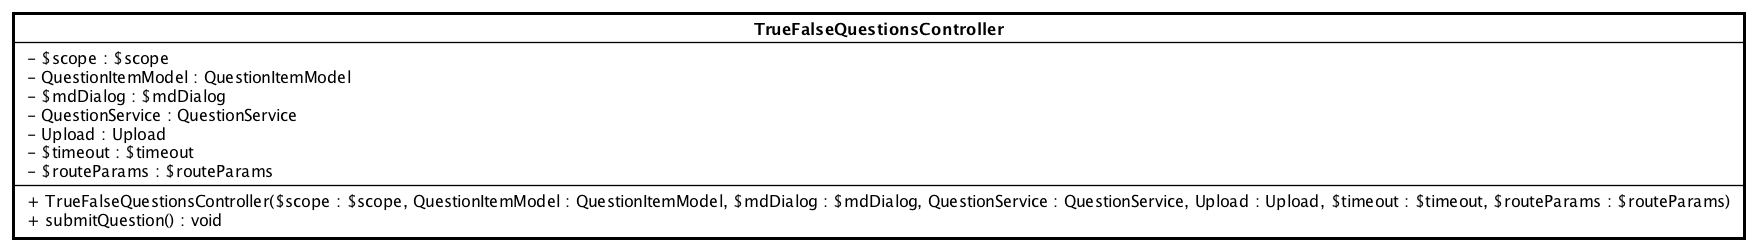
\includegraphics[scale=0.45]{UML/Classi/Front-End/QuizziPedia_Front-end_Controller_TrueFalseQuestionsController.png}
	\caption{QuizziPedia::Front-End::Controllers::TrueFalseQuestionsController}
\end{figure} \FloatBarrier
\begin{itemize}
	\item \textbf{Descrizione}: questa classe permette di gestire la creazione e la modifica di una domanda vero/falso;
	\item \textbf{Utilizzo}: fornisce le funzionalità per inserire una nuova domanda vero/falso nel database e per modificarne una esistente;
	\item \textbf{Relazione con altre classi}:
	\begin{itemize}
		\item \textit{IN} \texttt{TrueFalseQuestionsModelView}: ;
		\item \textit{IN} \texttt{QuestionService}: questa classe permette di ottenere domande esistenti e salvare nuove domande;
		\item \textit{IN} \texttt{QuestionItemModel}: è il modello (astratto) della domanda;
	\end{itemize}
	\item \textbf{Attributi}:
	\begin{itemize}
		\item \texttt{-} \texttt{\$scope: \$scope} \\
		Campo dati contenente un riferimento all’oggetto \$scope creato da \textit{Angular\ped{G}}, viene utilizzato come mezzo di comunicazione tra il controller e la view. Contiene gli oggetti che definiscono il model dell’applicazione;
		\item \texttt{-} \texttt{Question: QuestionItemModel} \\ Oggetto nel quale andremo a salvare la domanda dopo averla scaricata dal service (per poterla caricare nella view);
		\item \texttt{+} \texttt{\$cookie: \$cookie}: serve per recuperare l'id della domanda dalla pagina da cui arrivo;
		\item \texttt{-} \texttt{\$mdDialog: \$mdDialog} \\
		Campo dati contenente un riferimento al servizio della libreria \textit{Material for Angular\ped{G}} che permette di creare delle componenti a popup;
		\item \texttt{-} \texttt{QuestionService: QuestionService}: ;
	\end{itemize}
	\item \textbf{Metodi}:
	\begin{itemize}
		\item \texttt{+} \texttt{TrueFalseQuestionsController} \\ Costruttore della classe (controllerà anche se la domanda esiste (tramite cookie) e in caso la casica, altrimenti view con form vuota);
		\item \texttt{+} \texttt{submitQuestion}: raccoglie i dati dal modelview e li manda al service;
	\end{itemize}
\end{itemize}

\paragraph{QuizziPedia::Front-End::Controllers::MultipleQuestionsController}
\begin{figure} [ht]
	\centering
	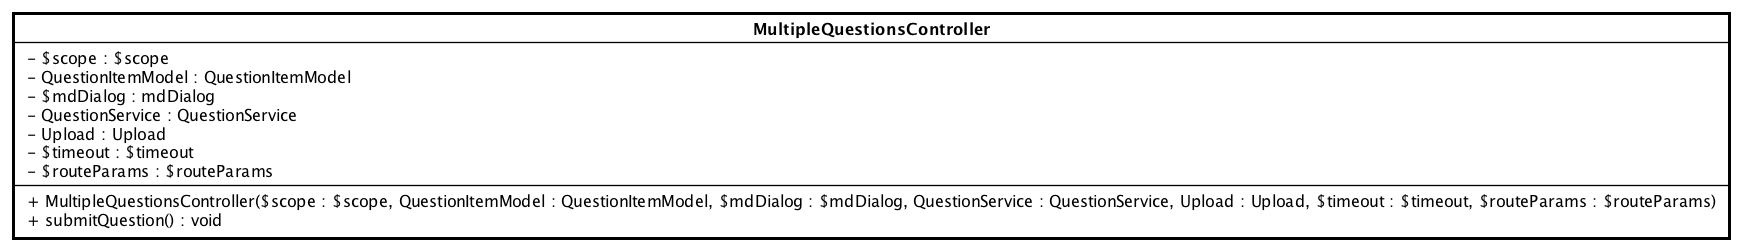
\includegraphics[scale=0.45]{UML/Classi/Front-End/QuizziPedia_Front-end_Controller_MultipleQuestionsController.png}
	\caption{QuizziPedia::Front-End::Controllers::MultipleChoiceQuestion}
\end{figure} \FloatBarrier
\begin{itemize}
	\item \textbf{Descrizione}: questa classe permette di gestire la creazione e la modifica di una domanda a risposta multipla;
	\item \textbf{Utilizzo}: fornisce le funzionalità per inserire una nuova domanda a risposta multipla nel database e per modificarne una esistente;
	\item \textbf{Relazione con altre classi}:
	\begin{itemize}
		\item \textit{IN} \texttt{MultipleQuestionsModelView}: ;
		\item \textit{IN} \texttt{QuestionService}: questa classe permette di ottenere domande esistenti e salvare nuove domande;
		\item \textit{IN} \texttt{QuestionItemModel}: è il modello (astratto) della domanda;
	\end{itemize}
	\item \textbf{Attributi}:
	\begin{itemize}
		\item \texttt{-} \texttt{\$scope: \$scope} \\
		Campo dati contenente un riferimento all’oggetto \$scope creato da \textit{Angular\ped{G}}, viene utilizzato come mezzo di comunicazione tra il controller e la view. Contiene gli oggetti che definiscono il model dell’applicazione;
		\item \texttt{-} \texttt{Question: QuestionItemModel} \\ Oggetto nel quale andremo a salvare la domanda dopo averla scaricata dal service (per poterla caricare nella view);
		\item \texttt{+} \texttt{\$cookie: \$cookie}: serve per recuperare l'id della domanda dalla pagina da cui arrivo;
		\item \texttt{-} \texttt{\$mdDialog: \$mdDialog} \\
		Campo dati contenente un riferimento al servizio della libreria \textit{Material for Angular\ped{G}} che permette di creare delle componenti a popup;
		\item \texttt{-} \texttt{QuestionService: QuestionService}: ;
	\end{itemize}
	\item \textbf{Metodi}:
	\begin{itemize}
		\item \texttt{+} \texttt{MultipleQuestionsController} \\ Costruttore della classe (controllerà anche se la domanda esiste (tramite cookie) e in caso la carica, altrimenti view con form vuota);
		\item \texttt{+} \texttt{submitQuestion}: raccoglie i dati dal modelview e li manda al service;
	\end{itemize}

\end{itemize}

\paragraph{QuizziPedia::Front-End::Controllers::ConnectionQuestionsController}
\begin{figure} [ht]
	\centering
	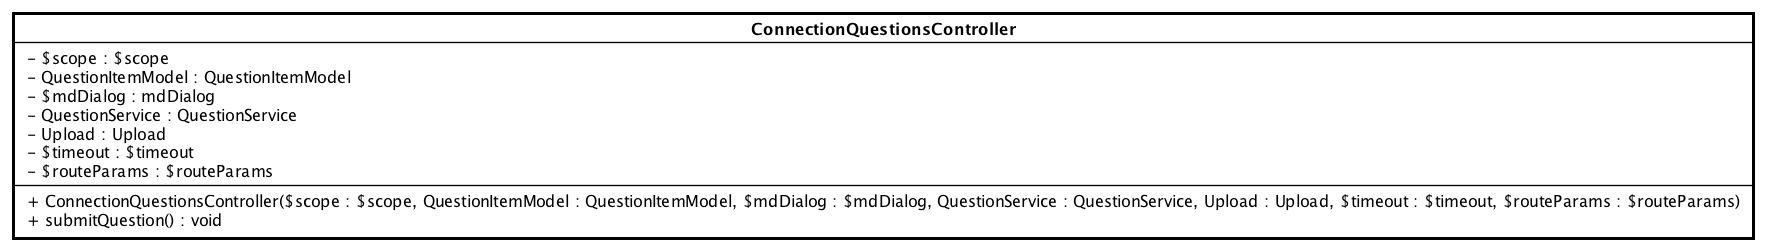
\includegraphics[scale=0.45]{UML/Classi/Front-End/QuizziPedia_Front-end_Controller_ConnectionQuestionsController.png}
	\caption{QuizziPedia::Front-End::Controllers::ConnectionQuestionsController}
\end{figure} \FloatBarrier
\begin{itemize}
	\item \textbf{Descrizione}: questa classe permette di gestire la creazione e la modifica di una domanda a collegamento;
	\item \textbf{Utilizzo}: fornisce le funzionalità per inserire una nuova domanda a collegamento nel database e per modificarne una esistente;
	\item \textbf{Relazione con altre classi}:
	\begin{itemize}
		\item \textit{IN} \texttt{ConnectionQuestionsModelView}: ;
		\item \textit{IN} \texttt{QuestionService}: questa classe permette di ottenere domande esistenti e salvare nuove domande;
		\item \textit{IN} \texttt{QuestionItemModel}: è il modello (astratto) della domanda;
	\end{itemize}
	\item \textbf{Attributi}:
	\begin{itemize}
		\item \texttt{-} \texttt{\$scope: \$scope} \\
		Campo dati contenente un riferimento all’oggetto \$scope creato da \textit{Angular\ped{G}}, viene utilizzato come mezzo di comunicazione tra il controller e la view. Contiene gli oggetti che definiscono il model dell’applicazione;
		\item \texttt{-} \texttt{Question: QuestionItemModel} \\ Oggetto nel quale andremo a salvare la domanda dopo averla scaricata dal service (per poterla caricare nella view);
		\item \texttt{+} \texttt{\$cookie: \$cookie}: serve per recuperare l'id della domanda dalla pagina da cui arrivo;
		\item \texttt{-} \texttt{\$mdDialog: \$mdDialog} \\
		Campo dati contenente un riferimento al servizio della libreria \textit{Material for Angular\ped{G}} che permette di creare delle componenti a popup;
		\item \texttt{-} \texttt{QuestionService: QuestionService}: ;
	\end{itemize}
	\item \textbf{Metodi}:
	\begin{itemize}
		\item \texttt{+} \texttt{ConnectionQuestionsController} \\ Costruttore della classe (controllerà anche se la domanda esiste (tramite cookie) e in caso la carica, altrimenti view con form vuota);
		\item \texttt{+} \texttt{submitQuestion}: raccoglie i dati dal modelview e li manda al service;
	\end{itemize}
\end{itemize}

\paragraph{QuizziPedia::Front-End::Controllers::ImagesSortingQuestionsController}
\begin{figure} [ht]
	\centering
	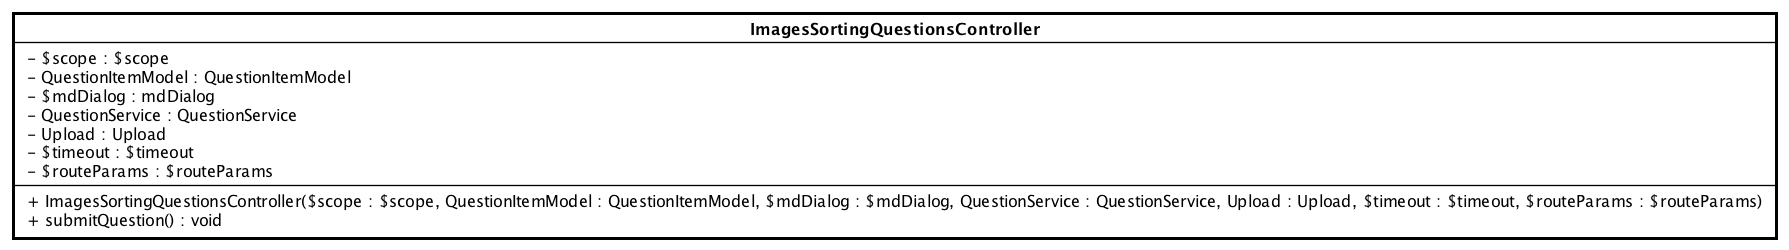
\includegraphics[scale=0.45]{UML/Classi/Front-End/QuizziPedia_Front-end_Controller_ImagesSortingQuestionsController.png}
	\caption{QuizziPedia::Front-End::Controllers::ImagesSortingQuestionsController}
\end{figure} \FloatBarrier
\begin{itemize}
	\item \textbf{Descrizione}: questa classe permette di gestire la creazione e la modifica di una domanda a ordinamento immagini;
	\item \textbf{Utilizzo}: fornisce le funzionalità per inserire una nuova domanda a ordinamento immagini nel database e per modificarne una esistente;
	\item \textbf{Relazione con altre classi}:
	\begin{itemize}
		\item \textit{IN} \texttt{ImageSortingQuestionsModelView}: ;
		\item \textit{IN} \texttt{QuestionService}: questa classe permette di ottenere domande esistenti e salvare nuove domande;
		\item \textit{IN} \texttt{QuestionItemModel}: è il modello (astratto) della domanda;
	\end{itemize}
	\item \textbf{Attributi}:
	\begin{itemize}
		\item \texttt{-} \texttt{\$scope: \$scope} \\
		Campo dati contenente un riferimento all’oggetto \$scope creato da \textit{Angular\ped{G}}, viene utilizzato come mezzo di comunicazione tra il controller e la view. Contiene gli oggetti che definiscono il model dell’applicazione;
		\item \texttt{-} \texttt{Question: QuestionItemModel} \\ Oggetto nel quale andremo a salvare la domanda dopo averla scaricata dal service (per poterla caricare nella view);
		\item \texttt{+} \texttt{\$cookie: \$cookie}: serve per recuperare l'id della domanda dalla pagina da cui arrivo;
		\item \texttt{-} \texttt{\$mdDialog: \$mdDialog} \\
		Campo dati contenente un riferimento al servizio della libreria \textit{Material for Angular\ped{G}} che permette di creare delle componenti a popup;
		\item \texttt{-} \texttt{QuestionService: QuestionService}: ;
	\end{itemize}
	\item \textbf{Metodi}:
	\begin{itemize}
		\item \texttt{+} \texttt{ImageSortingQuestionsController} \\ Costruttore della classe (controllerà anche se la domanda esiste (tramite cookie) e in caso la carica, altrimenti view con form vuota);
		\item \texttt{+} \texttt{submitQuestion}: raccoglie i dati dal modelview e li manda al service;
	\end{itemize}
\end{itemize}

\paragraph{QuizziPedia::Front-End::Controllers::StringsSortingQuestionsController}
\begin{figure} [ht]
	\centering
	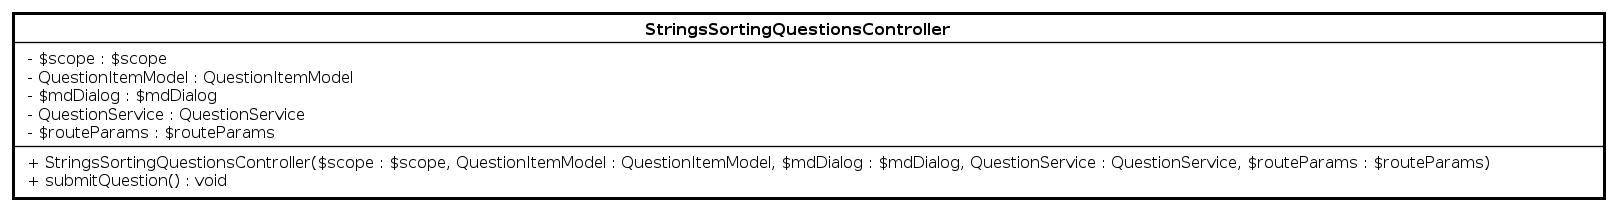
\includegraphics[scale=0.45]{UML/Classi/Front-End/QuizziPedia_Front-end_Controller_StringSortingQuestionsController.png}
	\caption{QuizziPedia::Front-End::Controllers::StringsSortingQuestionsController}
\end{figure} \FloatBarrier
\begin{itemize}
	\item \textbf{Descrizione}: questa classe permette di gestire la creazione e la modifica di una domanda a ordinamento di stringhe;
	\item \textbf{Utilizzo}: fornisce le funzionalità per inserire una nuova domanda a ordinamento di stringhe nel database e per modificarne una esistente;
	\item \textbf{Relazione con altre classi}:
	\begin{itemize}
		\item \textit{IN} \texttt{StringsSortingQuestionsModelView}: ;
		\item \textit{IN} \texttt{QuestionService}: questa classe permette di ottenere domande esistenti e salvare nuove domande;
		\item \textit{IN} \texttt{QuestionItemModel}: è il modello (astratto) della domanda;
	\end{itemize}
	\item \textbf{Attributi}:
	\begin{itemize}
		\item \texttt{-} \texttt{\$scope: \$scope} \\
		Campo dati contenente un riferimento all’oggetto \$scope creato da \textit{Angular\ped{G}}, viene utilizzato come mezzo di comunicazione tra il controller e la view. Contiene gli oggetti che definiscono il model dell’applicazione;
		\item \texttt{-} \texttt{Question: QuestionItemModel} \\ Oggetto nel quale andremo a salvare la domanda dopo averla scaricata dal service (per poterla caricare nella view);
		\item \texttt{+} \texttt{\$cookie: \$cookie}: serve per recuperare l'id della domanda dalla pagina da cui arrivo;
		\item \texttt{-} \texttt{\$mdDialog: \$mdDialog} \\
		Campo dati contenente un riferimento al servizio della libreria \textit{Material for Angular\ped{G}} che permette di creare delle componenti a popup;
		\item \texttt{-} \texttt{QuestionService: QuestionService}: ;
	\end{itemize}
	\item \textbf{Metodi}:
	\begin{itemize}
		\item \texttt{+} \texttt{StringsSortingQuestionsController} \\ Costruttore della classe (controllerà anche se la domanda esiste (tramite cookie) e in caso la carica, altrimenti view con form vuota);
		\item \texttt{+} \texttt{submitQuestion}: raccoglie i dati dal modelview e li manda al service;
	\end{itemize}
\end{itemize}

\paragraph{QuizziPedia::Front-End::Controllers::FillingQuestionsController}
\begin{figure} [ht]
	\centering
	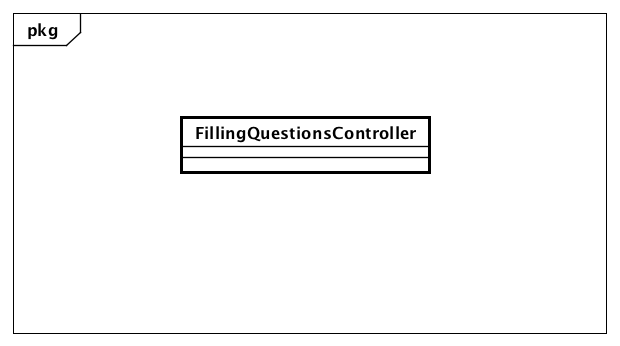
\includegraphics[scale=0.45]{UML/Classi/Front-End/QuizziPedia_Front-end_Controller_FillingQuestionsController.png}
	\caption{QuizziPedia::Front-End::Controllers::FillingQuestionsController}
\end{figure} \FloatBarrier
\begin{itemize}
	\item \textbf{Descrizione}: questa classe permette di gestire la creazione e la modifica di una domanda a riempimento di spazi;
	\item \textbf{Utilizzo}: fornisce le funzionalità per inserire una nuova domanda ariempimento di spazi nel database e per modificarne una esistente;
	\item \textbf{Relazione con altre classi}:
	\begin{itemize}
		\item \textit{IN} \texttt{FillingQuestionsModelView}: ;
		\item \textit{IN} \texttt{QuestionService}: questa classe permette di ottenere domande esistenti e salvare nuove domande;
		\item \textit{IN} \texttt{QuestionItemModel}: è il modello (astratto) della domanda;
	\end{itemize}
	\item \textbf{Attributi}:
	\begin{itemize}
		\item \texttt{-} \texttt{\$scope: \$scope} \\
		Campo dati contenente un riferimento all’oggetto \$scope creato da \textit{Angular\ped{G}}, viene utilizzato come mezzo di comunicazione tra il controller e la view. Contiene gli oggetti che definiscono il model dell’applicazione;
		\item \texttt{-} \texttt{Question: QuestionItemModel} \\ Oggetto nel quale andremo a salvare la domanda dopo averla scaricata dal service (per poterla caricare nella view);
		\item \texttt{+} \texttt{\$cookie: \$cookie}: serve per recuperare l'id della domanda dalla pagina da cui arrivo;
		\item \texttt{-} \texttt{\$mdDialog: \$mdDialog} \\
		Campo dati contenente un riferimento al servizio della libreria \textit{Material for Angular\ped{G}} che permette di creare delle componenti a popup;
		\item \texttt{-} \texttt{QuestionService: QuestionService}: ;
	\end{itemize}
	\item \textbf{Metodi}:
	\begin{itemize}
		\item \texttt{+} \texttt{FillingQuestionsController} \\ Costruttore della classe (controllerà anche se la domanda esiste (tramite cookie) e in caso la carica, altrimenti view con form vuota);
		\item \texttt{+} \texttt{submitQuestion}: raccoglie i dati dal modelview e li manda al service;
	\end{itemize}
\end{itemize}

\paragraph{QuizziPedia::Front-End::Controllers::ClickableAreaQuestionsController}
\begin{figure} [ht]
	\centering
	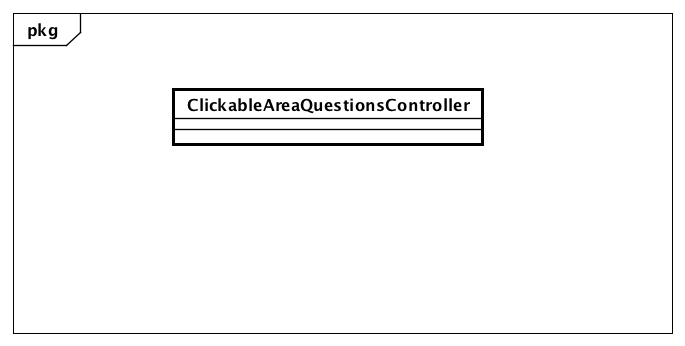
\includegraphics[scale=0.45]{UML/Classi/Front-End/QuizziPedia_Front-end_Controller_ClickableAreaQuestionsController.png}
	\caption{QuizziPedia::Front-End::Controllers::ClickableAreaQuestionsController}
\end{figure} \FloatBarrier
\begin{itemize}
	\item \textbf{Descrizione}: questa classe permette di gestire la creazione e la modifica di una domanda ad area cliccabile;
	\item \textbf{Utilizzo}: fornisce le funzionalità per inserire una nuova domanda ad area cliccabile nel database e per modificarne una esistente;
	\begin{itemize}
		\item \textit{IN} \texttt{ClickableAreaQuestionsModelView}: ;
		\item \textit{IN} \texttt{QuestionService}: questa classe permette di ottenere domande esistenti e salvare nuove domande;
		\item \textit{IN} \texttt{QuestionItemModel}: è il modello (astratto) della domanda;
	\end{itemize}
	\item \textbf{Attributi}:
	\begin{itemize}
		\item \texttt{-} \texttt{\$scope: \$scope} \\
		Campo dati contenente un riferimento all’oggetto \$scope creato da \textit{Angular\ped{G}}, viene utilizzato come mezzo di comunicazione tra il controller e la view. Contiene gli oggetti che definiscono il model dell’applicazione;
		\item \texttt{-} \texttt{Question: QuestionItemModel} \\ Oggetto nel quale andremo a salvare la domanda dopo averla scaricata dal service (per poterla caricare nella view);
		\item \texttt{+} \texttt{\$cookie: \$cookie}: serve per recuperare l'id della domanda dalla pagina da cui arrivo;
		\item \texttt{-} \texttt{\$mdDialog: \$mdDialog} \\
		Campo dati contenente un riferimento al servizio della libreria \textit{Material for Angular\ped{G}} che permette di creare delle componenti a popup;
		\item \texttt{-} \texttt{QuestionService: QuestionService}: ;
	\end{itemize}
	\item \textbf{Metodi}:
	\begin{itemize}
		\item \texttt{+} \texttt{ClickableAreaQuestionsController} \\ Costruttore della classe (controllerà anche se la domanda esiste (tramite cookie) e in caso la carica, altrimenti view con form vuota);
		\item \texttt{+} \texttt{submitQuestion}: raccoglie i dati dal modelview e li manda al service;
	\end{itemize}
\end{itemize}

\paragraph{QuizziPedia::Front-End::Controllers::EditorQMLController}
\begin{figure} [ht]
	\centering
	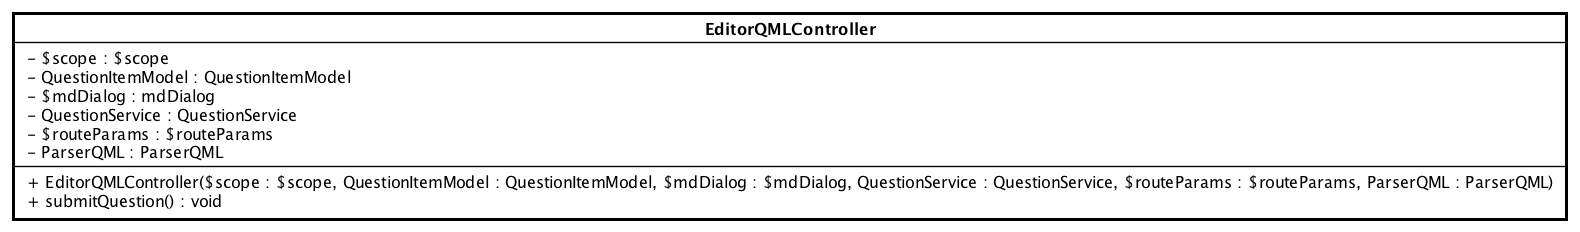
\includegraphics[scale=0.45]{UML/Classi/Front-End/QuizziPedia_Front-end_Controller_EditorQMLController.png}
	\caption{QuizziPedia::Front-End::Controllers::EditorQMLController}
\end{figure} \FloatBarrier
\begin{itemize}
	\item \textbf{Descrizione}: questa classe permette di gestire la creazione e la modifica di domande create tramite editor QML;
	\item \textbf{Utilizzo}: fornisce le funzionalità per creare e modificare una domanda tramite editor QML;
	\item \textbf{Relazione con altre classi}:
	\begin{itemize}
		\item \textit{IN} \texttt{EditorQMLView}: view contenente l'editor QML per la creazione di domande personalizzate; 
		\item \textit{OUT} \texttt{QuestionService}: questa classe permette di ottenere domande esistenti e salvare nuove domande;
	\end{itemize}
	\item \textbf{Attributi}:
	\begin{itemize}
		\item \texttt{-} \texttt{\$scope: \$scope} \\
		Campo dati contenente un riferimento all’oggetto \$scope creato da \textit{Angular\ped{G}}, viene utilizzato come mezzo di comunicazione tra il controller e la view. Contiene gli oggetti che definiscono il model dell’applicazione;
	\end{itemize}
	\item \textbf{Metodi}:
	\begin{itemize}
		\item 
	\end{itemize}
\end{itemize}

\paragraph{QuizziPedia::Front-End::Controllers::QuestionsManagementController}
\begin{figure} [ht]
	\centering
	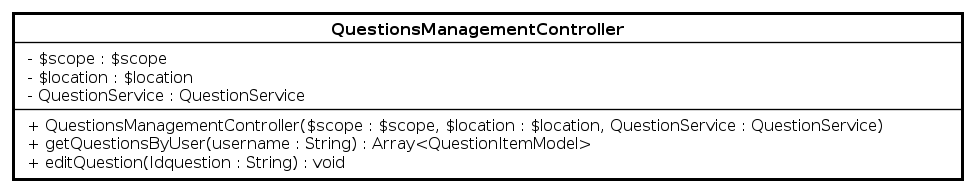
\includegraphics[scale=0.45]{UML/Classi/Front-End/QuizziPedia_Front-end_Controller_QuestionsManagementController.png}
	\caption{QuizziPedia::Front-End::Controllers::QuestionsManagementController}
\end{figure} \FloatBarrier
\begin{itemize}
	\item \textbf{Descrizione}: questa classe permette di gestire le domande create dall'utente e di crearne di nuove;
	\item \textbf{Utilizzo}: fornisce le funzionalità per richiedere al server le domande create dall'utente e mostrarle nella pagina dedicata. Inoltre permette di catturare gli eventi per modificare le domande esistenti e per crearne una di nuova; 
	\item \textbf{Relazione con altre classi}:
	\begin{itemize}
		\item \textit{IN} \texttt{QuestionsManagementModelView}: classe di tipo modelview la cui istanzazione è contenuta all'interno della variabile di ambiente \$scope di \textit{Angular.js\ped{G}}. All'interno di essa sono presenti le variabili e i metodi necessari per il \textit{Two-Way Data-Binding\ped{G}} tra la view \texttt{QuestionsManagementView} e il controller \texttt{QuestionsManagementController};; 
		\item \textit{IN} \texttt{QuestionService}: questa classe permette di ottenere domande esistenti e salvare nuove domande;
	\end{itemize}
	\item \textbf{Attributi}:
	\begin{itemize}
		\item \texttt{-} \texttt{\$scope: \$scope} \\
		Campo dati contenente un riferimento all’oggetto \$scope creato da \textit{Angular\ped{G}}, viene utilizzato come mezzo di comunicazione tra il controller e la view. Contiene gli oggetti che definiscono il model dell’applicazione;
		\item \texttt{-} \texttt{\$location: \$location} \\
		Campo dati contenente un riferimento al servizio creato da \textit{Angular\ped{G}} che permette di accedere alla barra degli indirizzi del \textit{browser\ped{G}}, i cambiamenti all’URL nella barra degli indirizzi si riflettono in questo oggetto e viceversa;
		\item \texttt{-} \texttt{QuestionService}\\
		Campo dati contenente un riferimento al servizio che si occupa della gestione delle informazioni legate alle domande;
	\end{itemize}
	\item \textbf{Metodi}:
	\begin{itemize}
		\item \texttt{+} \texttt{QuestionsManagementsController(\$scope: \$scope, \$location: \$location, QuestionService: QuestionService)} \\ 
		Metodo costruttore della classe; \\
		\textbf{Parametri}:
		\begin{itemize}
			\item \texttt{\$scope: \$scope} \\
			Parametro contenente un riferimento all’oggetto \$scope creato da \textit{Angular\ped{G}}. Viene utilizzato come mezzo di comunicazione tra il controller e la view. Contiene gli oggetti che definiscono il viewmodel e il model dell’applicazione;
			\item \texttt{\$location: \$location} \\
			Parametro contenente un riferimento al servizio creato da \textit{Angular\ped{G}} che permette di accedere alla barra degli indirizzi del \textit{browser\ped{G}}, i cambiamenti all’URL nella barra degli indirizzi si riflettono in questo oggetto e viceversa;
			\item \texttt{QuestionService: QuestionService} \\
			Parametro contenente un riferimento al servizio che si occupa della gestione delle informazioni legate alle domande;
		\end{itemize}
		\item \texttt{-} \texttt{getQuestionsByUser(username: String)} \\ 
		Metodo che acquisisce le domande create dall'utente attraverso il \texttt{QuestionService};\\
		\textbf{Parametri}:
		\begin{itemize}
			\item \texttt{username: String} \\
			Parametro di tipo \texttt{String} contenente l'username dell'utente;
		\end{itemize}
		\item \texttt{+} \texttt{editQuestion(idQuestion: String)} \\ 
		redirect a modifica domanda;
		\textbf{Parametri}:
		\begin{itemize}
			\item \texttt{idQuestion: username} \\
			Parametro di tipo \texttt{String} contenente l'id della domanda da modificare;
		\end{itemize}
	\end{itemize}
\end{itemize}

\paragraph{QuizziPedia::Front-End::Controllers::NewQuestionsButtonController}
\begin{figure} [ht]
	\centering
	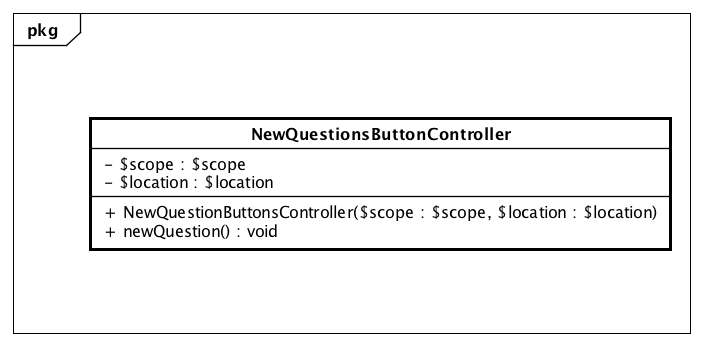
\includegraphics[scale=0.45]{UML/Classi/Front-End/QuizziPedia_Front-end_Controller_NewQuestionsButtonController.png}
	\caption{QuizziPedia::Front-End::Controllers::NewQuestionButtonController}
\end{figure} \FloatBarrier
\begin{itemize}
	\item \textbf{Descrizione}: questa classe permette di effettuare il redirect alla pagina di creazione nuova domanda;
	\item \textbf{Utilizzo}: effettua il redirect alla pagina di creazione nuova domanda quando l'utente seleziona l'apposito link;
	\item \textbf{Relazione con altre classi}:
	\begin{itemize}
		\item \textit{IN} \texttt{NewQuestionButtonsModelView}: ; 
	\end{itemize}
	\item \textbf{Attributi}:
	\begin{itemize}
		\item \texttt{-} \texttt{\$scope: \$scope} \\
		Campo dati contenente un riferimento all’oggetto \$scope creato da \textit{Angular\ped{G}}, viene utilizzato come mezzo di comunicazione tra il controller e la view. Contiene gli oggetti che definiscono il model dell’applicazione;
		\item \texttt{-} \texttt{\$location: \$location} \\
		Campo dati contenente un riferimento al servizio creato da \textit{Angular\ped{G}} che permette di accedere alla barra degli indirizzi del \textit{browser\ped{G}}, i cambiamenti all’URL nella barra degli indirizzi si riflettono in questo oggetto e viceversa;
	\end{itemize}
	\item \textbf{Metodi}:
	\begin{itemize}
		\item \texttt{+} \texttt{NewQuestionButtonsController()} \\ Metodo costruttore della classe;
		\item \texttt{+} \texttt{newQuestion()} \\ redirect a creazione domanda;
	\end{itemize}
\end{itemize}

\paragraph{QuizziPedia::Front-End::Controllers::StatisticsController}
\begin{figure} [ht]
	\centering
	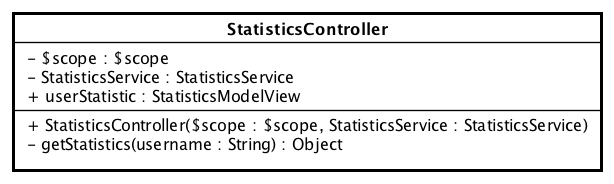
\includegraphics[scale=0.45]{UML/Classi/Front-End/QuizziPedia_Front-end_Controller_StatisticsController.png}
	\caption{QuizziPedia::Front-End::Controllers::StatisticsController}
\end{figure} \FloatBarrier
\begin{itemize}
	\item \textbf{Descrizione}: questa classe permette di le statistiche di un utente;
	\item \textbf{Utilizzo}: fornisce le funzionalità per ottenere le statistiche di un utente per poterle mostrare nella view;
	\item \textbf{Relazione con altre classi}:
	\begin{itemize}
		\item \textit{IN} \texttt{StatisticsModelView}: directive che permette di visualizzare le statistiche di un utente; 
		\item \textit{IN} \texttt{StatisticsService}: questa classe permette di ottenere le statistiche dell'utente;
		\item \textit{IN} \texttt{UserDetailsModel}: 
	\end{itemize}
	\item \textbf{Attributi}:
	\begin{itemize}
		\item \texttt{-} \texttt{\$scope: \$scope} \\
		Campo dati contenente un riferimento all’oggetto \$scope creato da \textit{Angular\ped{G}}, viene utilizzato come mezzo di comunicazione tra il controller e la view. Contiene gli oggetti che definiscono il model dell’applicazione;
		\item \texttt{-} \texttt{\$rootScope: \$rootScope} \\
		Campo dati contenente il riferimento all'oggetto globale \$rootScope creato da \textit{Angular\ped{G}}. Viene utilizzato per rendere accessibile a tutti i controller e a tutte le view l'oggetto \texttt{UserDetailsModel}. In questo caso viene utilizzato per inserire in \$rootScope l'oggetto di ritorno della chiamata a \texttt{getStatistics} del service \texttt{StatisticsService};
		\item \texttt{-} \texttt{StatisticsService}: parametro permette di ottenere le statistiche dell'utente;
	\end{itemize}	
	\begin{itemize}
		\item \textbf{Metodi}:
		\item \texttt{+} \texttt{StatisticsController()} \\ Metodo costruttore della classe;
		\item \texttt{-} \texttt{getStatistics(username: String)} \\ Metodo che permette di ottenere le statistiche con una chiamata a StatisticsService;
	\end{itemize}
\end{itemize}

\paragraph{QuizziPedia::Front-End::Controllers::MenuBarController}
\begin{figure} [ht]
	\centering
	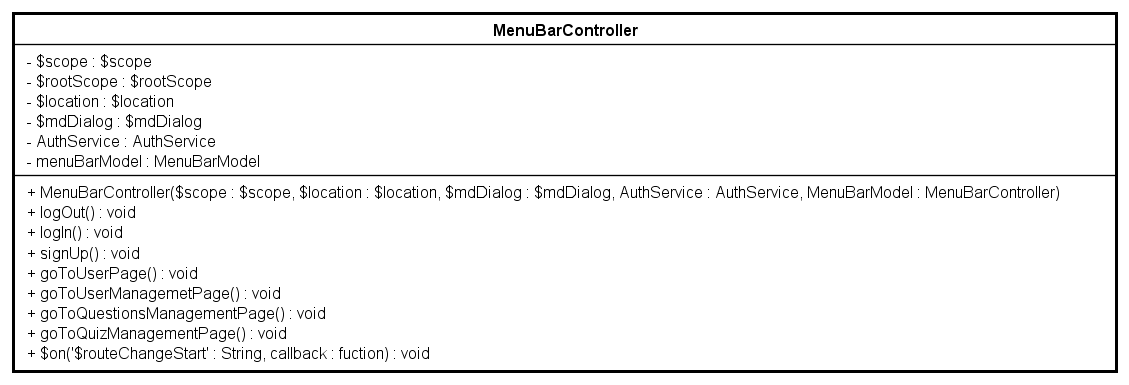
\includegraphics[scale=0.45]{UML/Classi/Front-End/QuizziPedia_Front-end_Controller_MenuBarController.png}
	\caption{QuizziPedia::Front-End::Controllers::MenuBarController}
\end{figure} \FloatBarrier
\begin{itemize}
	\item \textbf{Descrizione}: questa classe permette di gestire il menù fisso per ogni pagina;
	\item \textbf{Utilizzo}: fornisce le funzionalità per aggiornare, a seconda della pagina, il contenuto del menù;
	\item \textbf{Relazione con altre classi}:
	\begin{itemize}
		\item \textit{IN} \texttt{MenuBarDirective}: rappresenta il menù, presente in ogni pagina dell'applicazione, generato in base agli oggetti passati nello \$scope isolato. Fornisce un pulsante per ogni oggetto ricevuto come parametro, ogni pulsante viene rappresentato con un’icona e con un testo. Al click di un pulsante viene invocata la funzione ad esso associata;  
	\end{itemize}
	\item \textbf{Attributi}:
	\begin{itemize}
		\item \texttt{-} \texttt{\$scope: \$scope} \\
		Campo dati contenente un riferimento all’oggetto \$scope creato da \textit{Angular\ped{G}}, viene utilizzato come mezzo di comunicazione tra il controller e la view. Contiene gli oggetti che definiscono il model dell’applicazione;
	\end{itemize}
	\item \textbf{Metodi}:
	\begin{itemize}
		\item 
	\end{itemize}
\end{itemize}

\paragraph{QuizziPedia::Front-End::Controllers::LogoutController}
\begin{figure} [ht]
	\centering
	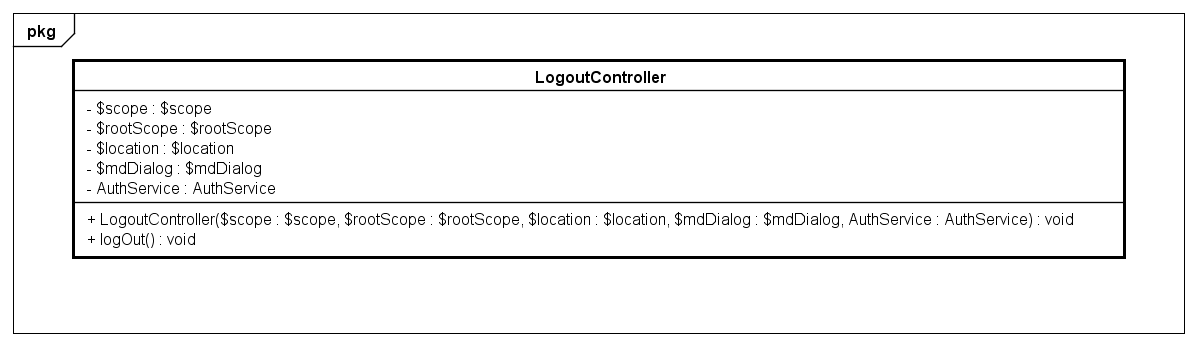
\includegraphics[scale=0.45]{UML/Classi/Front-End/QuizziPedia_Front-end_Controller_LogoutController.png}
	\caption{QuizziPedia::Front-End::Controllers::LogoutController}
\end{figure} \FloatBarrier
\begin{itemize}
	\item \textbf{Descrizione}: questa classe permette di gestire l'azione di logout;
	\item \textbf{Utilizzo}: fornisce la funzionalità per effettuare il logout dall'applicazione;
	\item \textbf{Relazione con altre classi}:
	\begin{itemize}
		\item \textit{OUT} \texttt{MenuBarModelView}: rappresenta il menù, presente in ogni pagina dell'applicazione, generato in base agli oggetti passati nello \$scope isolato. Fornisce un pulsante per ogni oggetto ricevuto come parametro, ogni pulsante viene rappresentato con un’icona e con un testo. Al click di un pulsante viene invocata la funzione ad esso associata. Nel caso di un utente autenticato sarà presente un bottone per effettuare il logout;
		\item \textit{IN} \texttt{AuthService}: questa classe permette di gestire la registrazione e l'autenticazione di un utente;
	\end{itemize}
	\item \textbf{Attributi}:
	\begin{itemize}
		\item \texttt{-} \texttt{\$scope: \$scope} \\
		Campo dati contenente un riferimento all’oggetto \$scope creato da \textit{Angular\ped{G}}. Viene utilizzato come mezzo di comunicazione tra il controller e la view. Contiene gli oggetti che definiscono il viewmodel e il model dell’applicazione;
		\item \texttt{-} \texttt{\$rootScope: \$rootScope} \\
		Campo dati contenente il riferimento all'oggetto globale \$rootScope creato da \textit{Angular\ped{G}}. Viene utilizzato per rendere accessibile a tutti i controller e a tutte le view l'oggetto \texttt{UserDetailsModel}. Nel caso della logout viene utilizzata per rimuovere da \$rootScope l'oggetto di di tipo \texttt{UsersDetailModel};
		\item \texttt{-} \texttt{\$location: \$location} \\
		Campo dati contenente un riferimento al servizio creato da \textit{Angular\ped{G}} che permette di accedere alla barra degli indirizzi del \textit{browser\ped{G}}, i cambiamenti all’URL nella barra degli indirizzi si riflettono in questo oggetto e viceversa;
		\item \texttt{-} \texttt{\$mdDialog: \$mdDialog} \\
		Campo dati contenente un riferimento al servizio della libreria \textit{Material for Angular\ped{G}} che permette di creare delle componenti a popup;
		\item \texttt{-} \texttt{AuthService: AuthService} \\
		Campo dati contenente un riferimento al servizio che si occupa della gestione delle informazioni legate all’autenticazione. Viene utilizzato il metodo \texttt{logOut} di \$texttt{AuthService} a cui viene passato il parametro \texttt{username};
	\end{itemize}
	\item \textbf{Metodi}:
	\begin{itemize}
		\item \texttt{+} \texttt{LogoutController(\$scope: \$scope, \$rootScope: \$rootScope, \$location: \$location, \$mdDialog: \$mdDialog, AuthService: AuthService)} \\
		Metodo costruttore della classe; \\
		\textbf{Parametri}:
		\begin{itemize}
			\item \texttt{\$scope: \$scope} \\
			Parametro contenente un riferimento all’oggetto \$scope creato da \textit{Angular\ped{G}}. Viene utilizzato come mezzo di comunicazione tra il controller e la view. Contiene gli oggetti che definiscono il viewmodel e il model dell’applicazione;
			\item \texttt{\$rootScope: \$rootScope} \\
			Parametro contenente il riferimento all'oggetto globale \$rootScope creato da \textit{Angular\ped{G}}. Viene utilizzato per rendere accessibile a tutti i controller e a tutte le view l'oggetto \texttt{UserDetailsModel}. Nel caso della logout viene utilizzata per rimuovere da \$rootScope l'oggetto di di tipo \texttt{UsersDetailModel};
			\item \texttt{\$location: \$location} \\
			Parametro contenente un riferimento al servizio creato da \textit{Angular\ped{G}} che permette di accedere alla barra degli indirizzi del \textit{browser\ped{G}}, i cambiamenti all’URL nella barra degli indirizzi si riflettono in questo oggetto e viceversa;
			\item \texttt{\$mdDialog: \$mdDialog} \\
			Parametro contenente un riferimento al servizio della libreria \textit{Material for Angular\ped{G}} che permette di creare delle componenti a popup;
			\item \texttt{AuthService: AuthService} \\
			Campo dati contenente un riferimento al servizio che si occupa della gestione delle informazioni legate all’autenticazione.  Viene utilizzato il metodo \texttt{logOut} di \$texttt{AuthService} a cui viene passato il parametro \texttt{username};
		\end{itemize}
		\item \texttt{+} \texttt{logOut(): void} \\
		Metodo che richiama il metodo \texttt{logOut} del service \texttt{AuthService} passandogli lo \texttt{username}. Prima di effettuare questa operazione viene mostrato a video un messaggio di conferma per il proseguo dell'operazione;
	\end{itemize}
\end{itemize}

\paragraph{QuizziPedia::Front-End::Controllers::FooterController}
\begin{figure} [ht]
	\centering
	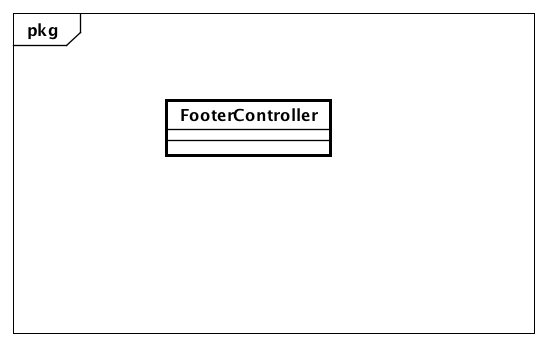
\includegraphics[scale=0.45]{UML/Classi/Front-End/QuizziPedia_Front-end_Controller_FooterController.png}
	\caption{QuizziPedia::Front-End::Controllers::FooterController}
\end{figure} \FloatBarrier
\begin{itemize}
	\item \textbf{Descrizione}: questa classe permette di gestire il footer dell'applicazione;
	\item \textbf{Utilizzo}: fornisce le funzionalità per recuperare le informazioni da mostrare nel footer;
	\item \textbf{Relazione con altre classi}:
	\begin{itemize}
		\item \textit{IN} \texttt{FooterDirective}: directive che mostra il footer dell'applicazione che sarà presente in ogni pagina;  
	\end{itemize}
	\item \textbf{Attributi}:
	\begin{itemize}
		\item \texttt{-} \texttt{\$scope: \$scope} \\
		Campo dati contenente un riferimento all’oggetto \$scope creato da \textit{Angular\ped{G}}, viene utilizzato come mezzo di comunicazione tra il controller e la view. Contiene gli oggetti che definiscono il model dell’applicazione;
	\end{itemize}
	\item \textbf{Metodi}:
	\begin{itemize}
		\item 
	\end{itemize}
\end{itemize}